\documentclass[a4paper]{article}
\usepackage[a4paper, left=2mm, right=2mm, top=5mm, bottom=5mm]{geometry}
\usepackage[utf8]{inputenc}
\usepackage[english,russian]{babel}
\usepackage{graphicx}
\usepackage{indentfirst}
\usepackage{amsmath}
\usepackage{floatflt}
\usepackage{enumerate}
\usepackage{amsfonts}
\usepackage{amssymb}
\title{Тепловая машина максимальной мощности\\(реферат)}
\author{С.~Е.~Володин, 272 гр.}
\date{}
\newcommand{\matrixl}{\left|\left|}
\newcommand{\matrixr}{\right|\right|}
\newcommand{\Tx}{$T_\text{х}$}
\newcommand{\Tn}{$T_\text{н}$}
\begin{document}
\maketitle
\section{Постановка задачи}
Фиксируем температуры нагревателя \Tn\ и холодильника \Tx. Требуется найти такую тепловую машину с временем цикла $t$ и полезной работой $A$, что максимальна ее мощность
$$
N=\frac{A}{t}.
$$
\section{Тепловая машина Карно и ее мощность}
Машина Карно обладает наибольшим КПД, но ее мощность равна нулю. Действительно, тепло получается и отдается на изотермах $T_{\text{н}}$ и $T_{\text{х}}$, что означает равенство температуры рабочего тела и температуры резервуара. Следовательно, поток тепла нулевой, значит, время прохождения изотермы бесконечно. Так как работа машины Карно конечна, получаем нулевую мощность:
$$
N^{\text{Карно}}=0.
$$
% картинка %
\section{Решение}
%\subsection{Необходимые условия}
\begin{floatingfigure}[l]{7cm}
%\begin{figure}[h]
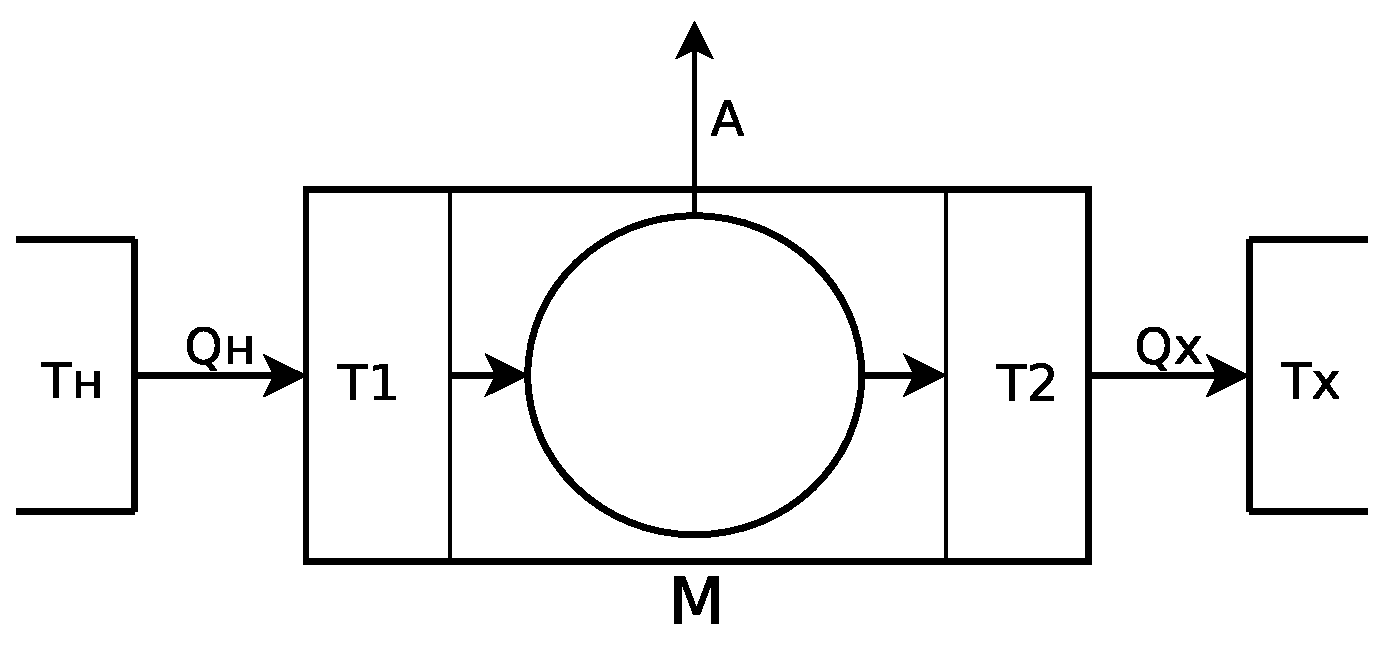
\includegraphics[width=6cm]{maxN}
%\caption{С}
%\end{figure}
\end{floatingfigure}
Разность температур между резервуаром и рабочим телом должна быть ненулевой (иначе $N=0$).\newline
Если теплоемкости рабочего тела или резервуара конечны, то в процессе теплообмена разность температур будет уменьшаться, что приведет к уменьшению теплового потока, и, следовательно, к увеличению времени (и уменьшению мощности). Поэтому теплоемкости должны быть бесконечны, и разности температур $\Delta T_\text{н}=T_\text{н}-T_1$ и $\Delta T_\text{х}=T_2-T_\text{х}$ постоянны.\newline
Также в качестве тепловой машины $M$ необходимо использовать машину Карно, так как у других машин меньший КПД, и, следовательно, меньшая работа $A$ при том же времени $t$.
% картинка %
\subsection{Поиск оптимальных разниц температур $\Delta T_\text{н}$ и $\Delta T_\text{х}$}
Считаем, что теплообмен осуществляется в соответствии с законом Фурье:
$$
Q_\text{н}=\varkappa S\frac{\Delta T_{\text{н}}}{L}t_{\text{н}},\ 
Q_\text{х}=\varkappa S\frac{\Delta T_{\text{х}}}{L}t_{\text{х}},\ 
\text{где}
\begin{array}{l}
L\text{~--- расстояние между рабочим телом и резервуаром во время теплообмена},\\
S\text{~--- площадь контакта},\\
\varkappa\text{~--- коэффициент теплопроводности среды.}
\end{array}
$$
Так как используется машина Карно,
%$\frac{T_1}{T_2}=\frac{Q_{\text{н}}}{Q_{\text{х}}}$.\newline
$T1/T2=Q_{\text{н}}/Q_{\text{х}}$.\newline
Выразим мощность, считая, что временем прохождения адиабат можно пренебречь:
$$
N=\frac{A}{t}=\frac{Q_\text{н}-Q_\text{х}}{t_{\text{н}}+t_{\text{х}}}=
\frac{\varkappa S}{L}\Delta T_{\text{н}}\frac{1-\frac{T_2}{T_1}}{1+\frac{T_2}{T_1}\frac{\Delta T_{\text{н}}}{\Delta T_{\text{х}}}}=
\frac{\varkappa S}{L}\Delta T_{\text{н}}\Delta T_{\text{х}}\frac{T_{\text{н}}-T_{\text{х}}-\Delta T_{\text{н}}-\Delta T_{\text{х}}}{T_{\text{н}}\Delta T_{\text{х}}+T_{\text{х}}\Delta T_{\text{н}}}=
\frac{\varkappa S(T_{\text{н}}-T_{\text{х}})^2}{LT_{\text{н}}}\left[\frac{1-x-y}{y+\beta x}xy\right],
\begin{array}{lcr}
x=\Delta T_{\text{н}}/(T_{\text{н}}-T_{\text{х}}),\\
%y=\frac{\Delta T_{\text{х}}}{T_{\text{н}}-T_{\text{х}}},\\
y=\Delta T_{\text{х}}/(T_{\text{н}}-T_{\text{х}}),\\
%\beta= \frac{T_{\text{х}}}{T_{\text{н}}}
\beta= T_{\text{х}}/T_{\text{н}}.
\end{array}
$$
%где $x=\frac{\Delta T_{\text{н}}}{T_{\text{н}}-T_{\text{х}}},\ y=\frac{\Delta T_{\text{х}}}{T_{\text{н}}-T_{\text{х}}},\ \beta= \frac{T_{\text{х}}}{T_{\text{н}}} $\newline 
То есть, нужно найти максимум функции $f(x,y)=\frac{1-x-y}{y+\beta x}xy$ при $
\left\{
\begin{array}{l}
x>0\\
y>0\\
1-x-y>0\\
\end{array}	
\right.
.
$\newline
Расчет, проведенный в п. \ref{maxsection}, дает
$x_0=\frac{1}{2(1+\sqrt{\beta})},\ y_0=\frac{\sqrt{\beta}}{2(1+\sqrt{\beta})},$\newline
{\Large\fbox{$\eta=1-\sqrt{\frac{T_{\text{х}}}{T_{\text{н}}}}$},
\fbox{$N^{max}=\frac{\varkappa S}{4L}(\sqrt{T_{\text{н}}}-\sqrt{T_{\text{х}}})^2$}.}
\newpage
\section{Максимум $f(x,y)$}
\label{maxsection}
$f\geq 0$, а на границе ограничений $f=0$. Обозначим $\alpha=\frac{y}{x}$ и найдем максимум на луче $\alpha=const$:\newline
$
f_\alpha(x)=\alpha x \frac{1-x-\alpha x}{\alpha + \beta},\ \frac{df_\alpha(x_0)}{dx}=\alpha x \frac{1-x-\alpha x}{\alpha + \beta}=0 \Longrightarrow x_0=\frac{1}{2(1+\alpha)}$.\newline
$f_\alpha(x_0)=\frac{\alpha}{\alpha + \beta}\frac{1}{4(1+\alpha)},\ 
\frac{df_\alpha(x_0)}{d\alpha}(\alpha_0)=0\Longrightarrow (1+\alpha)(\alpha+\beta)-\alpha(2\alpha+\beta+1)=0\Longrightarrow\alpha=\sqrt{\beta},\ 
x_0=\frac{1}{2(1+\sqrt{\beta})},\ y_0=\frac{\sqrt{\beta}}{2(1+\sqrt{\beta})}.$\newline
Отсюда\newline
$ %\begin{array}{l}
\Delta T_{\text{н}}=\frac{1}{2}\sqrt{T_{\text{н}}}(\sqrt{T_{\text{н}}}-\sqrt{T_{\text{х}}}),\ 
\Delta T_{\text{х}}=\frac{1}{2}\sqrt{T_{\text{х}}}(\sqrt{T_{\text{н}}}-\sqrt{T_{\text{х}}});
%\end{array}
$\newline 
$
%\begin{array}{l}
T_1=T_{\text{н}}-\Delta T_{\text{н}}=\frac{1}{2}(T_{\text{н}}+\sqrt{T_{\text{н}}T_{\text{х}}}),\ 
T_2=T_{\text{х}}+\Delta T_{\text{х}}=\frac{1}{2}(T_{\text{х}}+\sqrt{T_{\text{н}}T_{\text{х}}});
%\end{array}
$\newline
$\frac{T_2}{T_1}=\sqrt{\frac{T_{\text{х}}}{T_{\text{н}}}};$\newline
$f_{\alpha_0}(x_0)=\frac{1}{4(1+\sqrt{\beta})^2};$\newline
$N^{max}=\frac{\varkappa S(T_{\text{н}}-T_{\text{х}})^2}{LT_{\text{н}}}\frac{1}{4}\frac{T_{\text{н}}}{(\sqrt{T_{\text{н}}}+\sqrt{T_{\text{х}}})^2}=
\frac{\varkappa S}{4L}(\sqrt{T_{\text{н}}}-\sqrt{T_{\text{х}}})^2$

\begin{thebibliography}{0}
\bibitem{b1} Булыгин В. С. Некоторые задачи теории теплопроводности
\bibitem{b2} Булыгин В. С. Теоремы Карно
\end{thebibliography}


\end{document}
